\section{Results}
\label{sec:Results}

As proof of concept, the prototype of L.U.N.A sphere for 3D mapping using the concept impulse out of conservation of angular momentum as a unidirectional drive to roll a 2D laser scanner in an IMU equipped, pose-tracked spherical robot system, has been build and tested successfully. Potential for improvement and technical limitations have been identified.
The resulting sphere is shown in fig. \ref{sec:TechnicalApproach:fig:setup}
\begin{figure}
\centering                                                                                                                                                                                                        
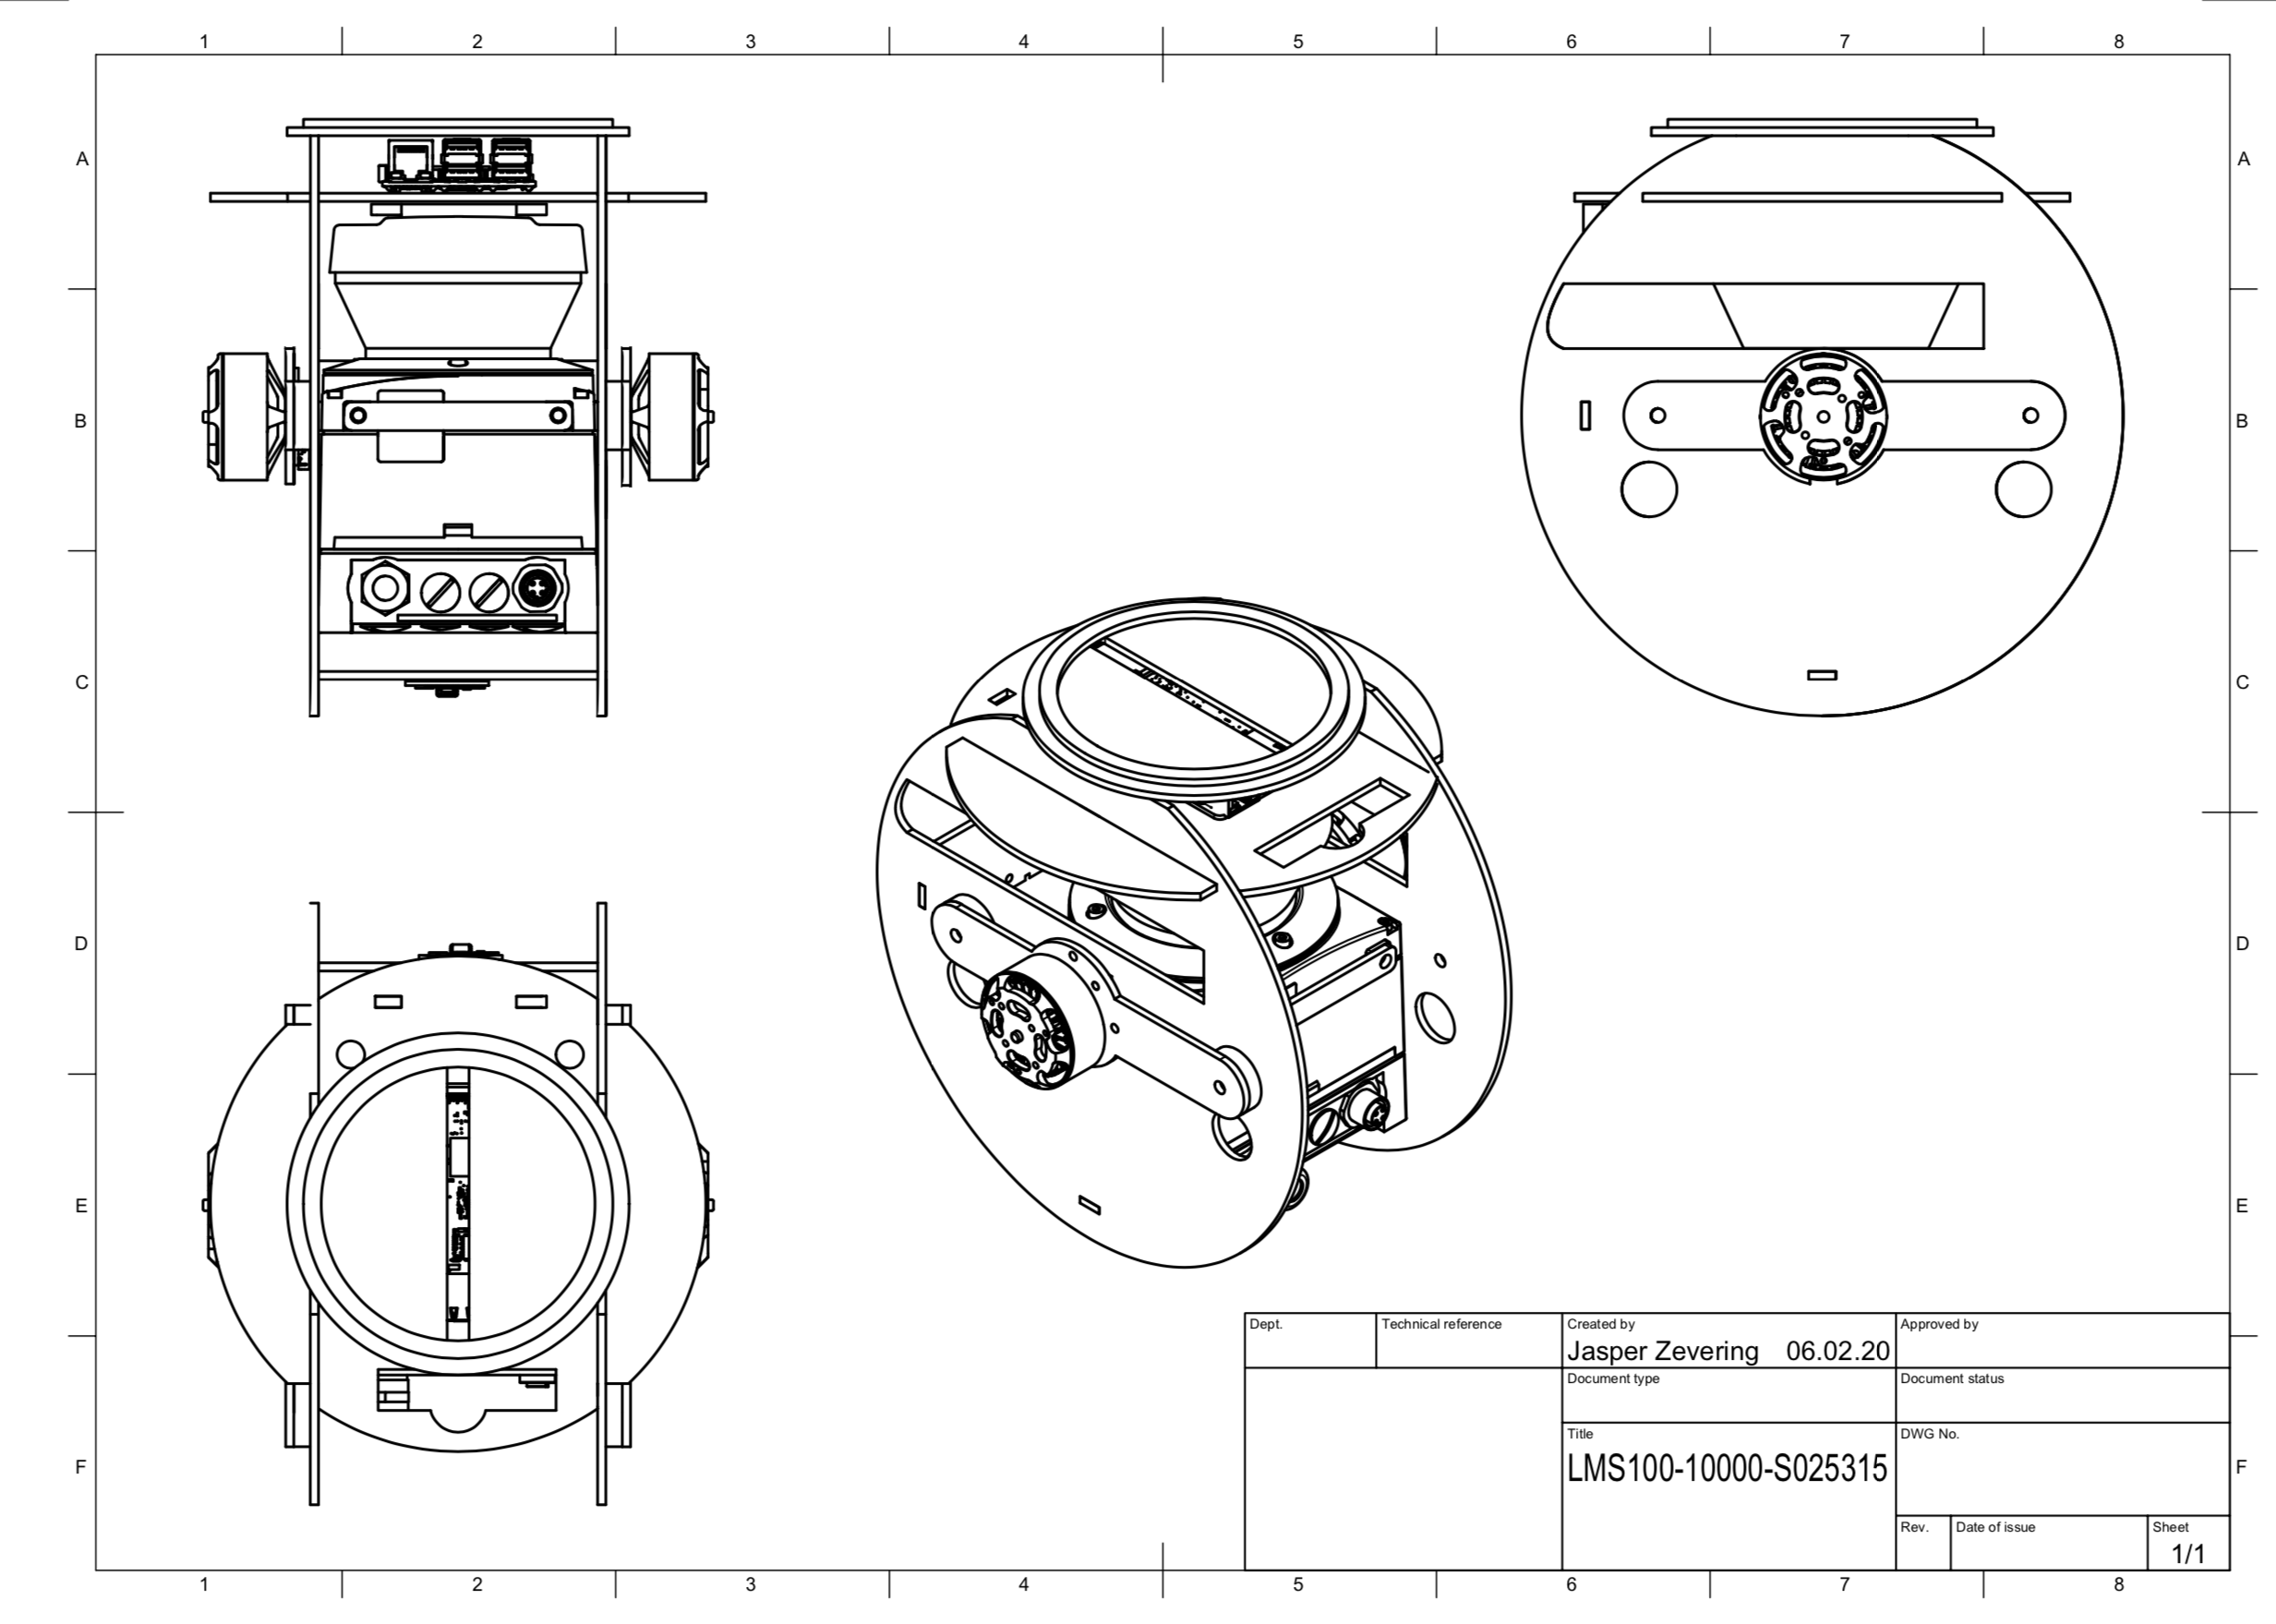
\includegraphics[height=50mm]{../Media/BlueprintPNG.png}                                                                                                                                                      
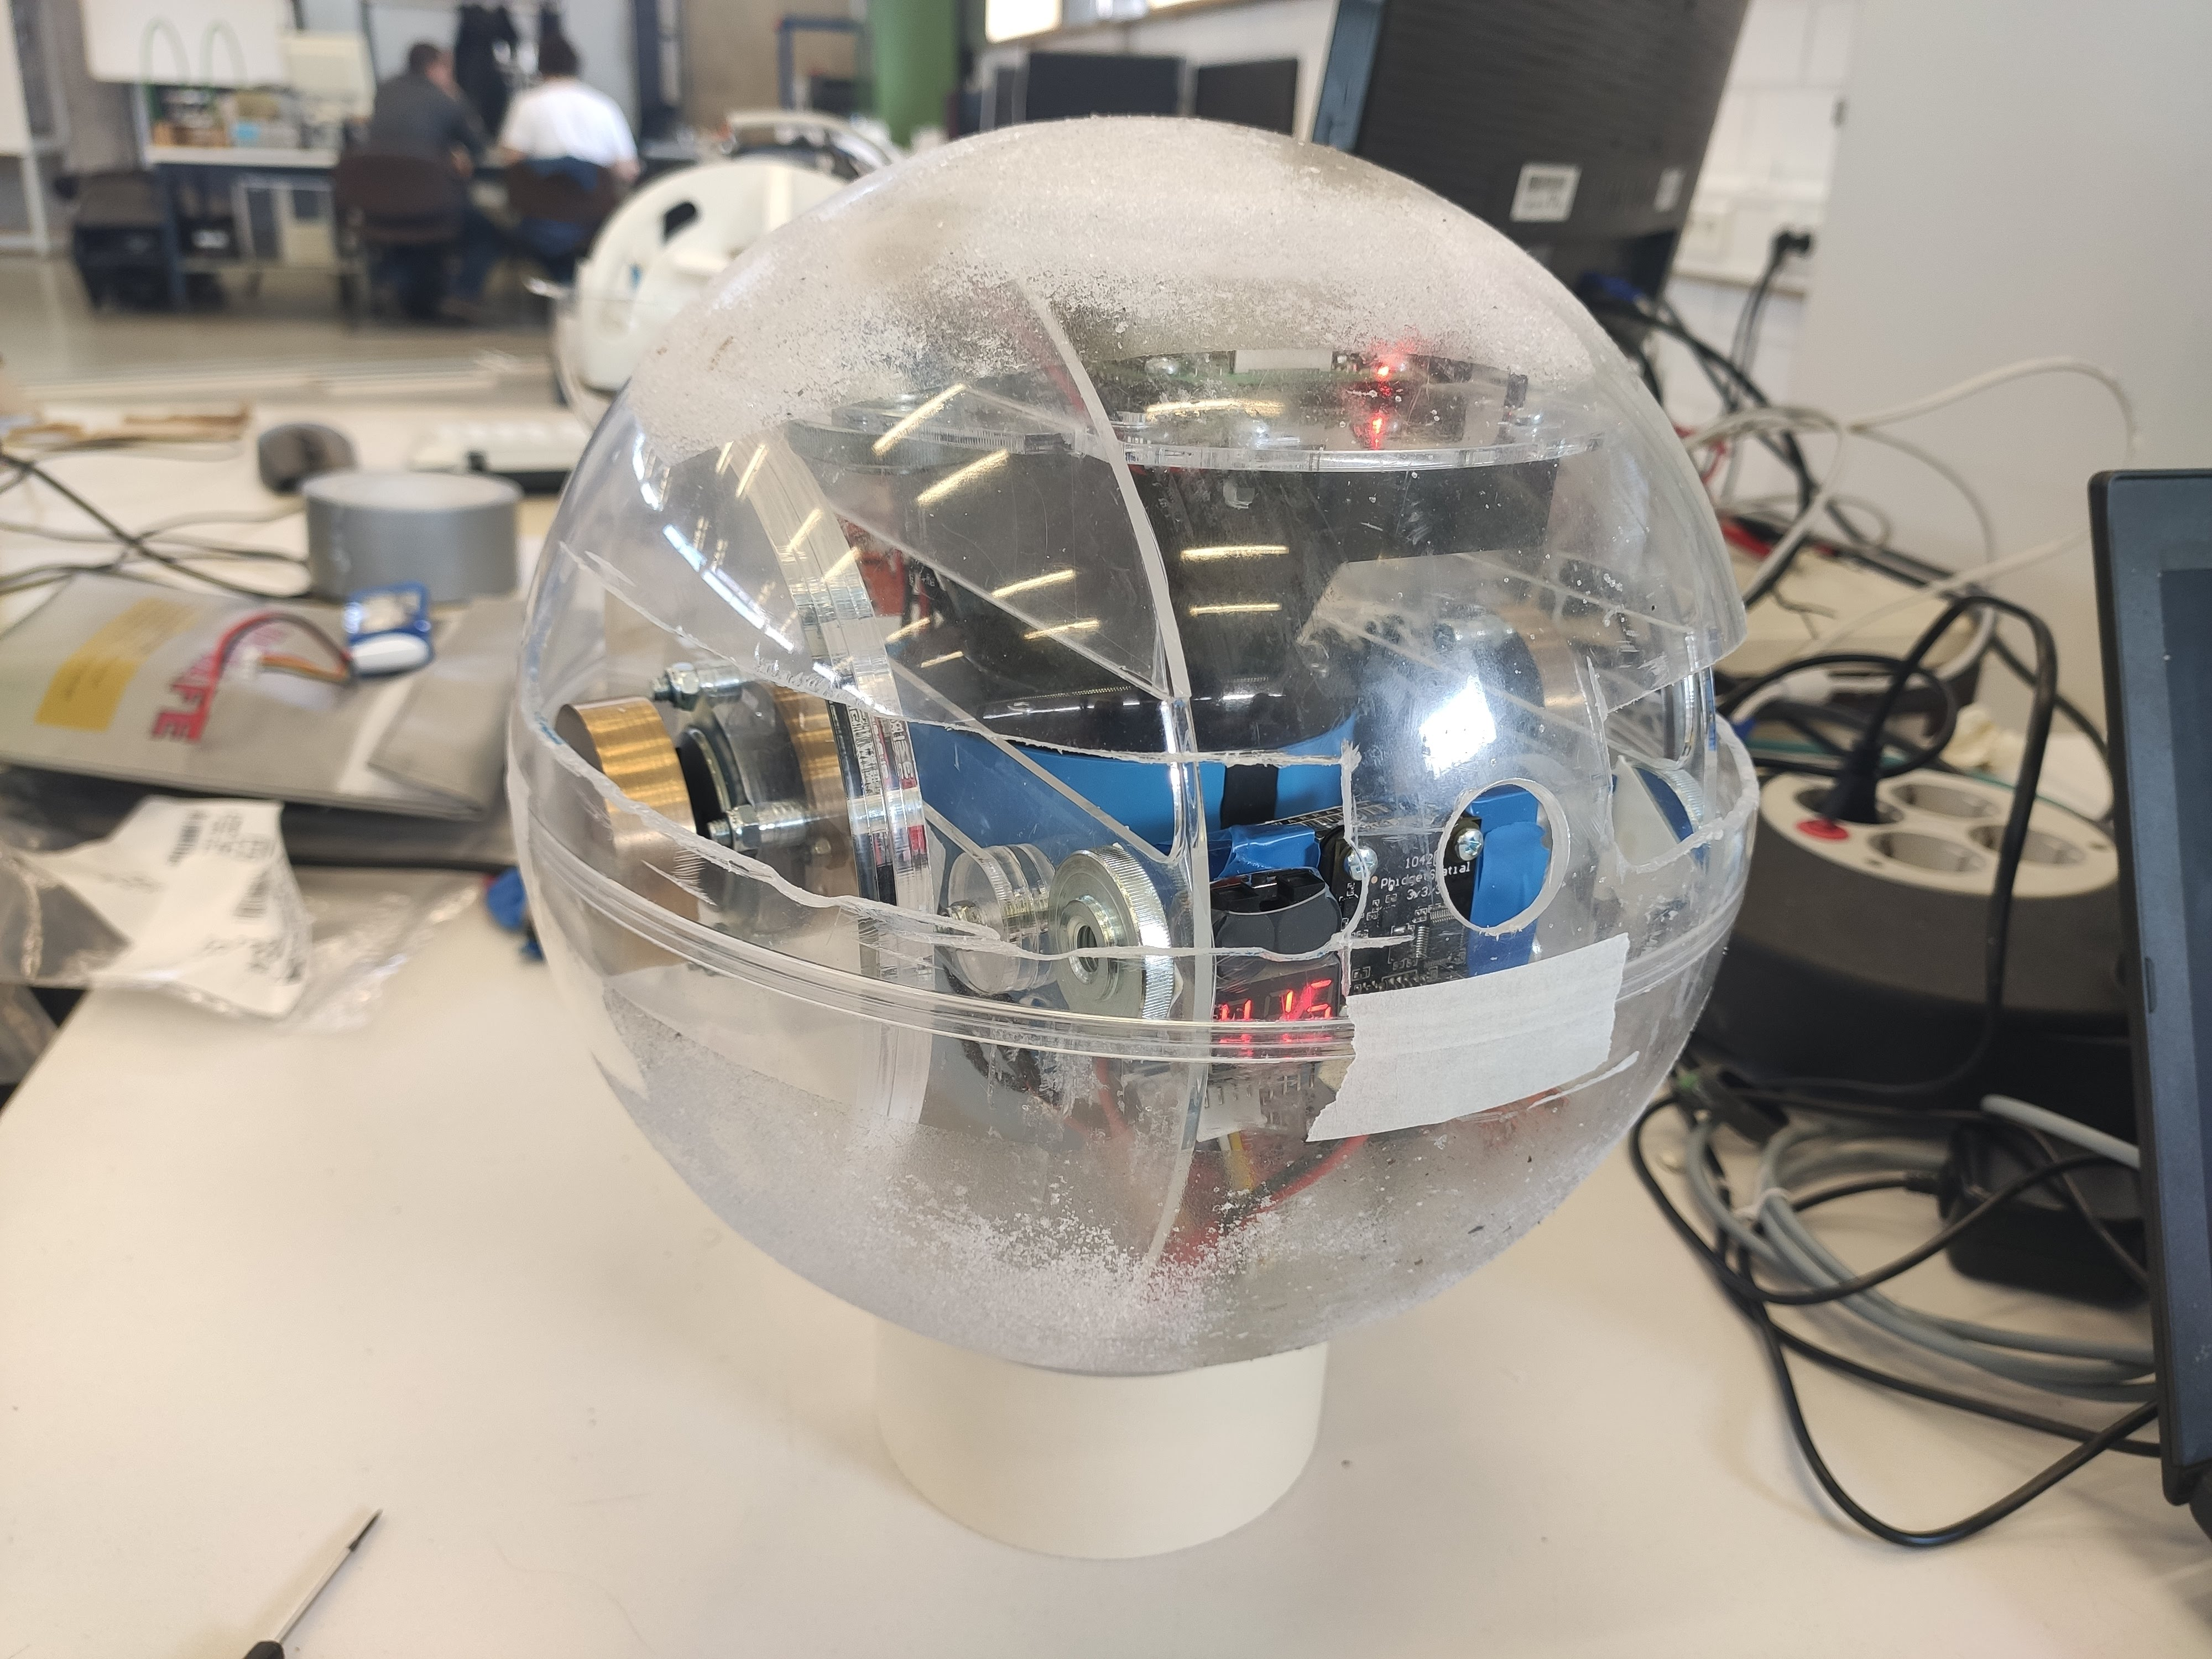
\includegraphics[height=50mm]{../Media/sphereFullshellLeft.jpg}
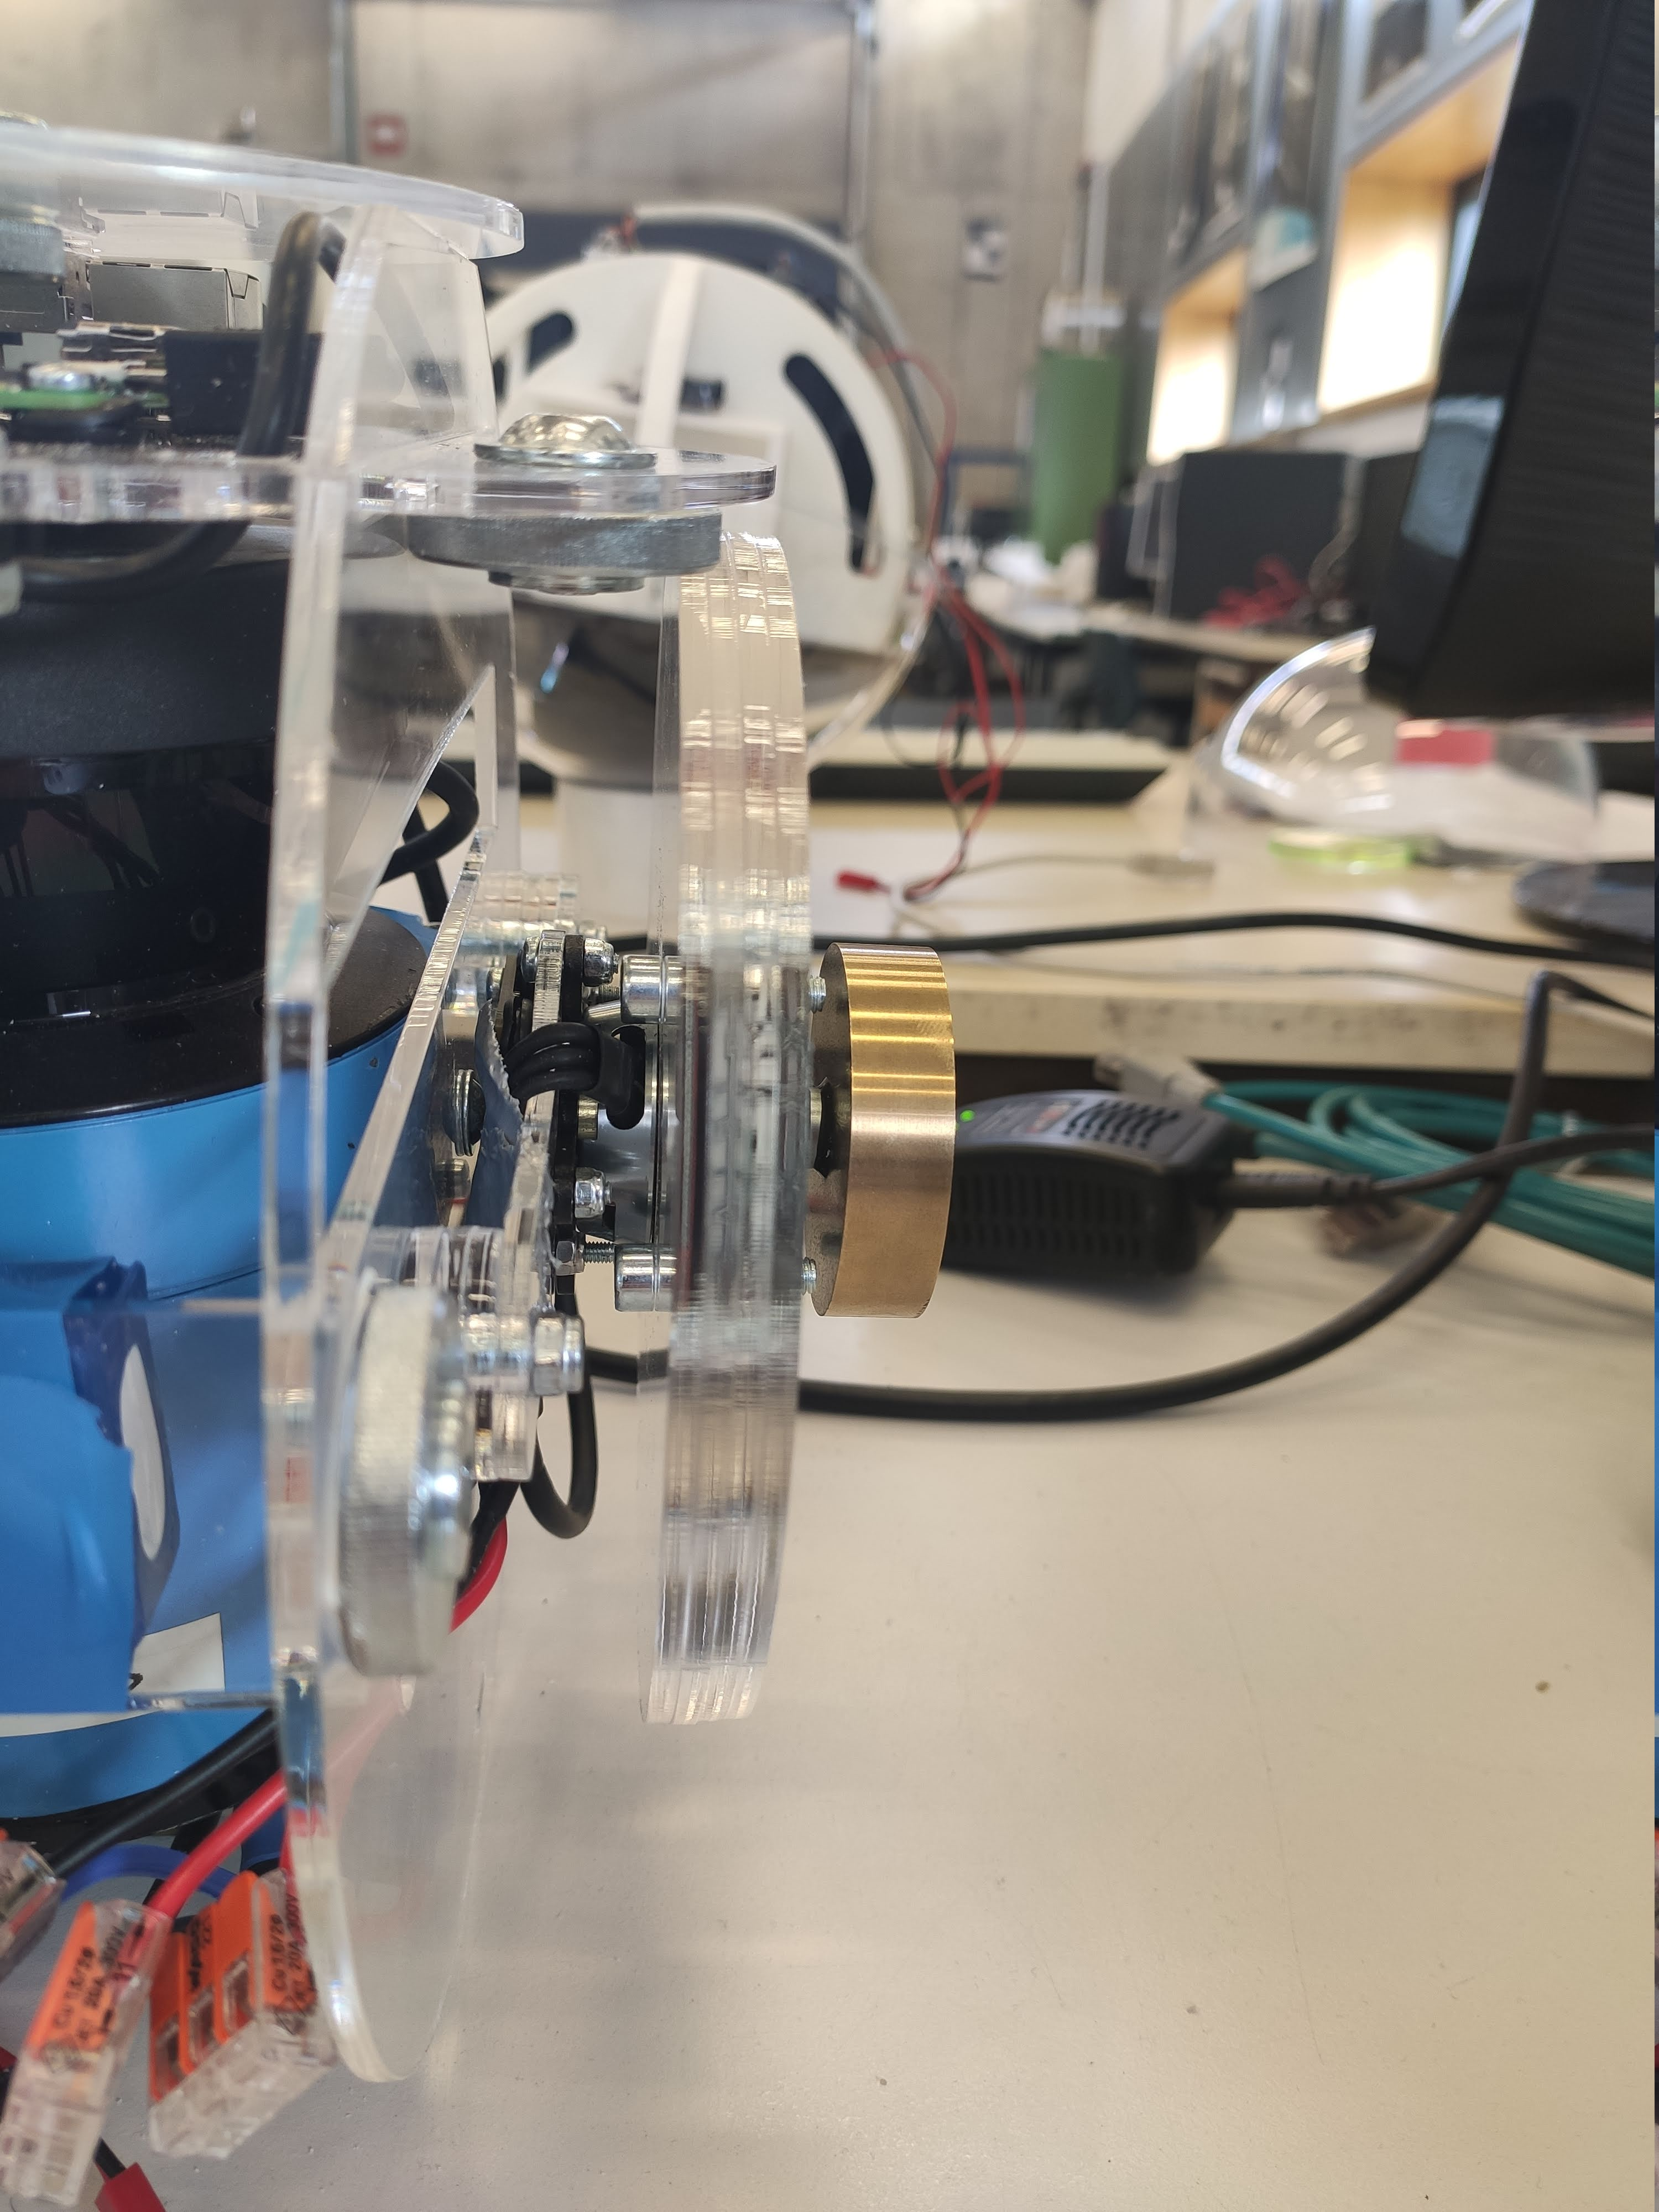
\includegraphics[height=50mm]{../Media/sphereRightMotor.jpg}   
\begin{subfigure}[b]{0.32\textwidth}
	\centering
	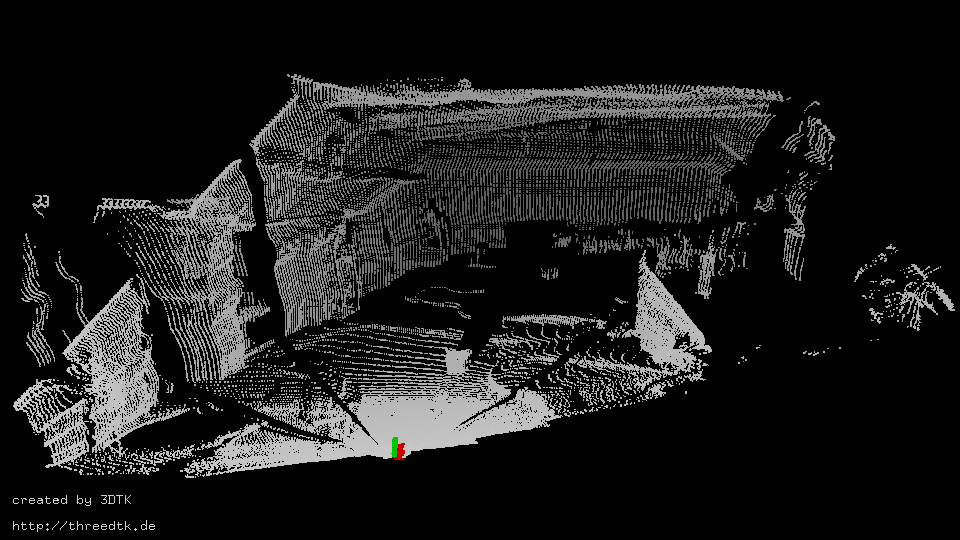
\includegraphics[width=\textwidth]{../Media/FirstDecentMap}
	\caption{Test with limited movement and no exterior shell.}
	\label{sec:experimentalResults:3DLaserScanning:fig:firstpointcloud}
\end{subfigure}
\begin{subfigure}[b]{0.32\textwidth}
	\centering
	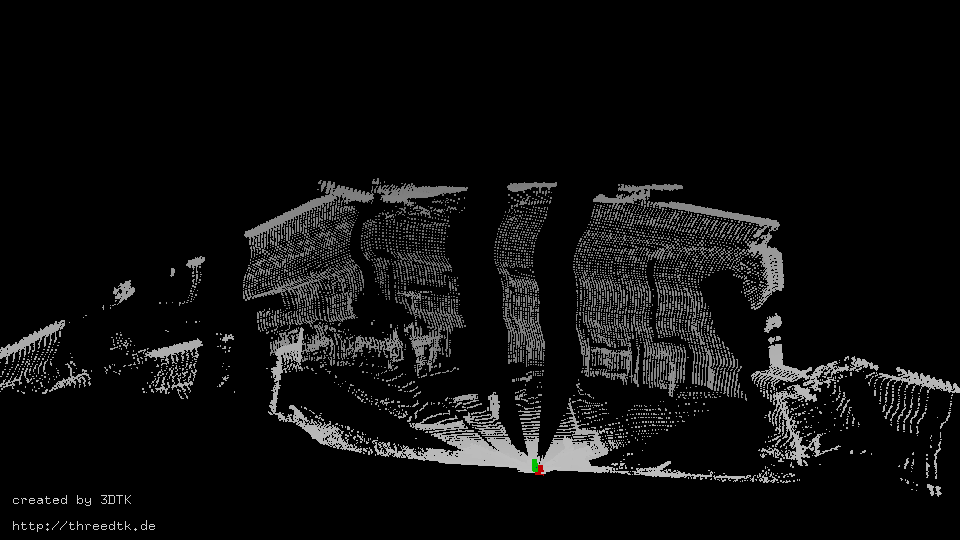
\includegraphics[width=\textwidth]{../Media/testScanWithTop}
	\caption{Test with limited movement and exterior shell.}
	\label{sec:experimentalResults:3DLaserScanning:fig:secondpointcloud}
\end{subfigure}
\begin{subfigure}[b]{0.32\textwidth}
	\centering
	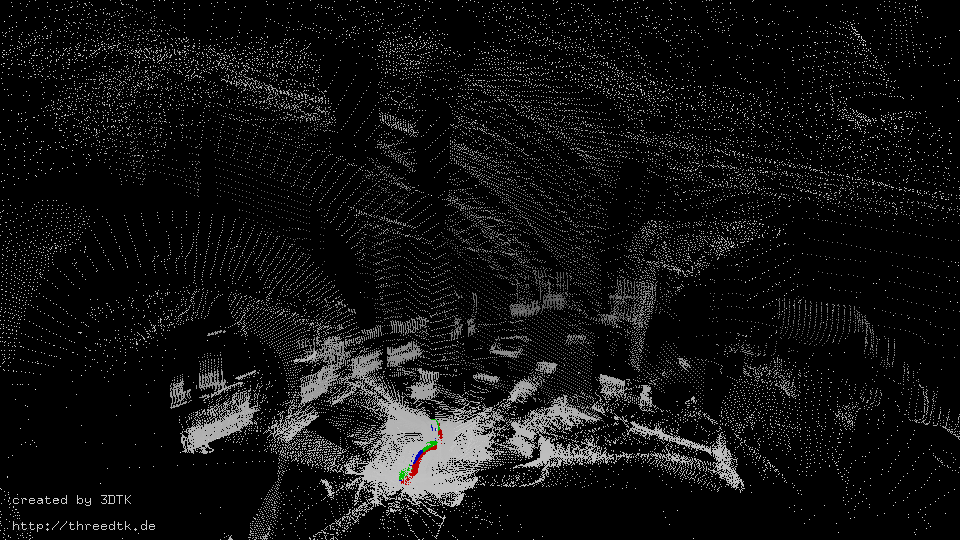
\includegraphics[width=\textwidth]{../Media/RollingTestMap}
	\caption{Test with exterior shell and full movement.}
	\label{sec:experimentalResults:3DLaserScanning:fig:thirdpointcloud}
\end{subfigure}
\caption{Hardware setup and laser-scanning Results of the L.U.N.A sphere prototype The Hardware including notches in the shell and friction granule (middle left). IMU (beneath supporting structure) and brushless motor  including flywheel mass (above supporting structure)(middle right).}
\label{sec:TechnicalApproach:fig:setup}

\end{figure}